\begin{center}
\begin{figure}[ht]
\begin{center}
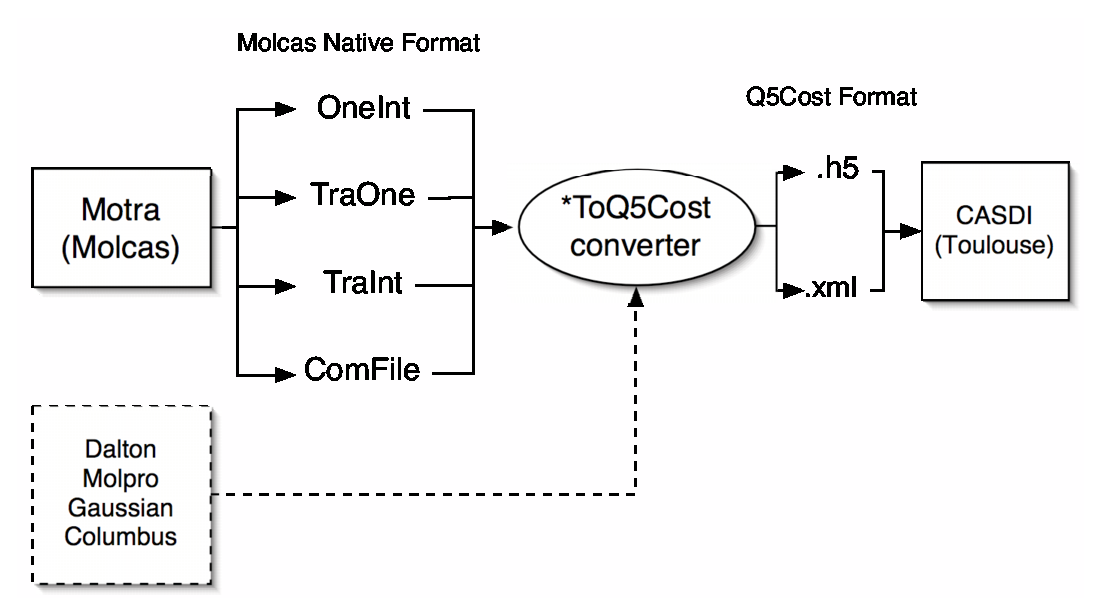
\includegraphics[width=10cm,keepaspectratio]{04_grid/images/q5cost-final-gimped.eps}
\end{center}
\caption{\footnotesize One of the possible final code layouts, involving
direct changes in the code. An integral producer, such as \texttt{MOLCAS}, provides
proprietary files. These files are fed to a converter, which creates the new
Q5Cost format. The program \texttt{CASDI} from Toulouse directly reads these
files. This infrastructure at the moment is not possible, because the
current \texttt{CASDI} implementation reads the old COST format.}
\label{fig:q5cost-final}
\end{figure}
\end{center}
